Handle theory is a powerful tool in differential topology.
Its main idea is to use \term{handles}
as basic building blocks for manifolds,
just like cells are building blocks for CW complexes.

\begin{definition}
    Let $0\leq\lambda\leq n$ be integers.
    A \term{$\lambda$-handle} of dimension $n$ 
    is a thickened version of the $\lambda$-disk:
    \[ h^\lambda := D^\lambda \times D^{n-\lambda}. \]
    It is an $n$-dimensional manifold, possibly with corners. \varqed
\end{definition}

For example, for $n=3$, the different types of handles are depicted below.
\[ 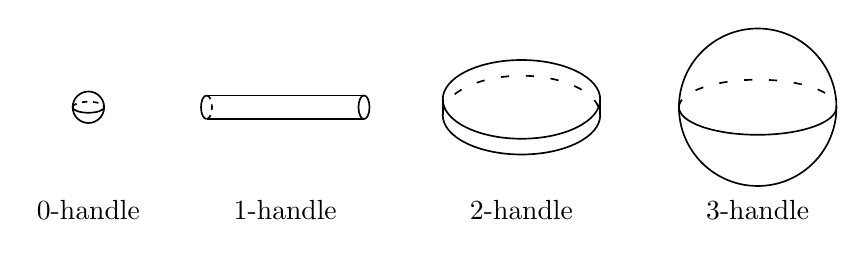
\begin{tikzpicture}[line width=.6, baseline=(base.base)]
    \tikzstyle{dp}=[dash pattern=on 2pt off 2pt]
    \draw (0,0) circle (.2);
    \draw[dp] (-.2,0) arc (180 : 0 : .2 and .07);
    \draw (-.2,0) arc (180 : 360 : .2 and .07);
    \node at (0,-1.3) {\text{$0$-handle}};
    
    \draw (1.5,.15) arc (90 : 270 : .07 and .15);
    \draw[dp] (1.5,.15) arc (90 : -90 : .07 and .15);
    \draw (3.5,0) ellipse (.07 and .15);
    \draw (1.5,.15) -- (3.5,.15) (1.5,-.15) -- (3.5,-.15);
    \node at (2.5,-1.3) {\text{$1$-handle}};

    \draw (5.5,.1) ellipse (1 and .5);
    \draw[loosely dashed] (4.5,-.1) arc (180 : 0 : 1 and .5);
    \draw (4.5,-.1) arc (180 : 360 : 1 and .5);
    \draw (4.5,.1) -- (4.5,-.1) (6.5,.1) -- (6.5,-.1);
    \node at (5.5,-1.3) {\text{$2$-handle}};

    \draw (8.5,0) circle (1);
    \draw[loosely dashed] (7.5,0) arc (180 : 0 : 1 and .35);
    \draw (7.5,0) arc (180 : 360 : 1 and .35);
    \node (base) at (8.5,-1.3) {\text{$3$-handle}};
\end{tikzpicture} \]

Every manifold can be obtained from $0$-handles
by attaching other handles.
For example, the solid torus $D^2 \times S^1$
decomposes into a $0$-handle and a $1$-handle.
\[ 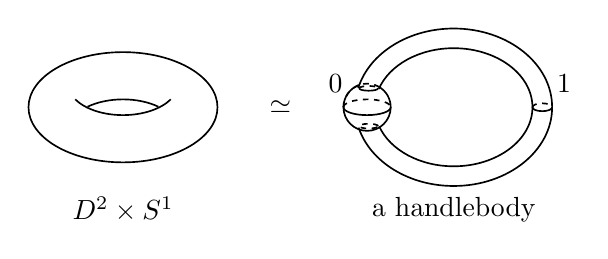
\begin{tikzpicture}[line width=.6]
    \tikzstyle{dp}=[dash pattern=on 2pt off 2pt]
    \draw (0,0) ellipse (1.2 and .7);
    \draw (0,-.1) arc (-90 : -30 : .7 and .4);
    \draw (0,-.1) arc (-90 : -150 : .7 and .4);
    \draw (0,.1) arc (90 : 50 : .7 and .4);
    \draw (0,.1) arc (90 : 130 : .7 and .4);
    
    \node at (2,0) {\text{$\simeq$}};

    \draw[dp] (2.8,0) arc (180 : 50 : .3);
    \draw (2.8,0) arc (180 : 110 : .3);
    \draw (2.8,0) arc (180 : 420 : .3);
    \draw[dp] (2.8,0) arc (180 : 0 : .3 and .1);
    \draw (2.8,0) arc (180 : 360 : .3 and .1);

    \draw (5.45,0) arc (0 : 166 : 1.25 and 1);
    \draw (5.45,0) arc (0 : -165 : 1.25 and 1);
    \draw (5.2,0) arc (0 : 162 : 1 and .75);
    \draw (5.2,0) arc (0 : -161 : 1 and .75);

    \draw[dp] (3,.24) arc (180 : 0 : .12 and .03);
    \draw (3,.24) arc (180 : 360 : .12 and .03);
    \draw[dp] (3.12,-.24) ellipse (.12 and .03);
    \draw[dp] (5.2,0) arc (180 : 0 : .125 and .05);
    \draw (5.2,0) arc (180 : 360 : .125 and .05);

    \node at (0,-1.3) {\text{$D^2 \times S^1$}};
    \node at (4.2,-1.3) {\text{a handlebody}};
    \node at (2.7,.3) {\text{0}};
    \node at (5.6,.3) {\text{1}};
\end{tikzpicture} \]

A formal definition goes as follows.

\begin{definition}
    A \term{relative $n$-handlebody} is a sequence
    \[ A = N_0 \subset N_1 \subset \cdots \]
    of smooth $n$-manifolds, possibly with boundary,
    such that each $N_i$ is obtained from $N_{i-1}$
    by attaching a $\lambda$-handle:
    \[ N_i \simeq N_{i-1} \cup_{\Phi_i} h^\lambda, \]
    where $\lambda$ may vary with $i$, and the attaching map
    \[ \Phi_i \: \partial D^\lambda \times D^{n-\lambda} \to \partial N_{i-1} \]
    is a smooth embedding.
    We require local finiteness (see below), so that the space
    \[ N := \bigcup_i N_i \]
    is a smooth $n$-manifold.

    By abuse of language,
    the pair $(N,A)$ is called a \term{relative $n$-handlebody}.
    If $A=\emptyset$, then $N$ is called an \term{$n$-handlebody}.
    It is \term{finite} if the above sequence is finite. \varqed
\end{definition}

In this definition, \term{local finiteness} means that 
every point in $N$ has a neighbourhood that intersects 
with only finitely many handles.
This is needed to ensure that $N$ is a manifold.

This definition is not completely rigorous,
since attaching a handle will form corners on the manifold,
and one needs to eliminate them in each step.
For details, the reader is referred to \cite{wall}.

The handlebody was invented by Smale,
and played a magical role in his proof of the
generalised Poincar\'e conjecture \cite{smale}.

\begin{theorem}[Generalised Poincar\'e conjecture]
    If $n\geq6$, then every smooth $n$-manifold
    homotopy equivalent to the $n$-sphere
    is homeomorphic to the $n$-sphere.
\end{theorem}

Note that ``homeomorphic'' can not be improved to ``diffeomorphic'',
since there exist different smooth structures on $S^7$.

The main step of the proof was the following.

\begin{theorem}[$h$-cobordism theorem]
    Suppose $M,N,W$ are simply connected compact manifolds, with $\dim W\geq6$ and 
    \[ \partial W = M \sqcup N. \]
    If the inclusions $M\hookrightarrow W$ and $N\hookrightarrow W$
    are homotopy equivalences, then there is a diffeomorphism
    \[ W \simeq M \times [0,1]. \]
\end{theorem}

\begin{proof}[Sketch of Proof]
    The proof of this theorem relies on the theory of handlebodies.
    We first decompose $W$ into handles,
    regarding it as obtained from $M$ by attaching handles.
    For dimensional reasons, $M$ is replaced by $M\times[0,1]$,
    which is a neighbourhood of $M$ in $W$.
    Then we manipulate these handles using the following two theorems.
    It turns out that everything can be cancelled out perfectly,
    leading to the desired diffeomorphism.
\end{proof}

The two theorems that were used in the proof 
of the $h$-cobordism theorem are the following.

\begin{theorem}[Rearrangement] \label{thm-rearrangement}
    Every finite handlebody can be rearranged,
    so that every $\lambda$-handle is attached on handles
    of type $<\lambda$.
\end{theorem}

\[ 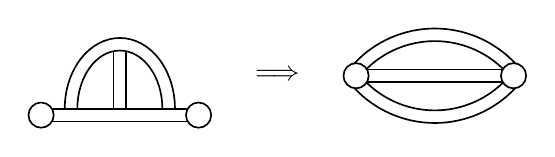
\begin{tikzpicture}[line width=.6]
    \draw (0,0) circle (.16);
    \draw (2,0) circle (.16);
    \draw (.14,.08) -- (1.86,.08) (.14,-.08) -- (1.86,-.08);
    \draw (.3,.08) arc (180 : 0 : .7 and .9);
    \draw (.46,.08) arc (180 : 0 : .54 and .74);
    \draw (.92,.08) -- (.92,.82) (1.08,.08) -- (1.08,.82);

    \node at (3,.5) {\text{$\Longrightarrow$}};

    \draw (4,.5) circle (.16);
    \draw (6,.5) circle (.16);
    \draw (4.14,.58) -- (5.86,.58) (4.14,.42) -- (5.86,.42);
    \draw (5,1.1) arc (90 : 137 : 1.4);
    \draw (5,1.1) arc (90 : 43 : 1.4);
    \draw (5,.94) arc (90 : 134 : 1.24);
    \draw (5,.94) arc (90 : 46 : 1.24);
    \draw (5,-.1) arc (-90 : -137 : 1.4);
    \draw (5,-.1) arc (-90 : -43 : 1.4);
    \draw (5,.06) arc (-90 : -134 : 1.24);
    \draw (5,.06) arc (-90 : -46 : 1.24);
\end{tikzpicture} \]

To be more precise,
it is convenient to introduce some terminology here.
(They are invented by the author and not meant to be used elsewhere.)

\begin{definition}
    Two $n$-handlebodies are \term{similar}
    if their manifolds $N$ are diffeomorphic, and for every $\lambda$,
    they have the same number of $\lambda$-handles. \varqed
\end{definition}

For example, the two handlebodies shown in the above picture are similar.

\begin{definition}
    A handlebody is \term{good} if 
    every $\lambda$-handle is attached on handles of type $<\lambda$. \varqed
\end{definition}

Thus, the rearrangement theorem can be reformulated as follows.

{
    \def\thetheorem{\ref*{thm-rearrangement}′}
    \begin{theorem}[Rearrangement]
        Every finite handlebody is similar to a good one.
    \end{theorem}
    \addtocounter{theorem}{-1}
}

The other theorem allows handles to cancel.

\begin{definition}
    The \term{belt} of the handle $D^\lambda \times D^{n-\lambda}$
    is $\{0\}\times \partial D^{n-\lambda}$,
    and the \term{cobelt} is $\partial D^\lambda\times\{0\}$.
    They are subsets of the boundary of the handle. \varqed
\end{definition}

\begin{theorem}[Cancellation]
    Suppose that 
    \[ N \cup h^\lambda \cup h^{\lambda+1} \]
    is a handlebody obtained from $N$ by attaching two handles.
    If the cobelt of $h^{\lambda+1}$ intersects the belt of $h^\lambda$
    in exactly one point,
    then the new handlebody is diffeomorphic to $N$.
\end{theorem}

\[ 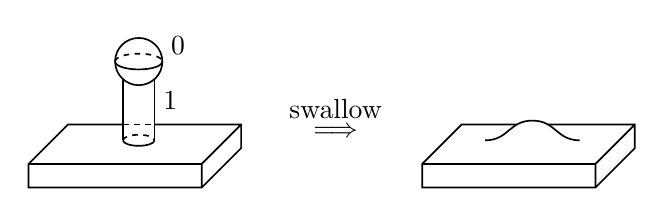
\begin{tikzpicture}[line width=.6]
    \tikzstyle{dp}=[dash pattern=on 2pt off 2pt]
    
    \draw (-.2,.2) -- (-.9,.2) -- (-1.4,-.3) -- (-1.4,-.6) -- (.8,-.6) -- (1.3,-.1) -- (1.3,.2) -- (.2,.2)
          (-1.4,-.3) -- (.8,-.3) -- (1.3,.2)
          (.8,-.3) -- (.8,-.6);
    \draw[dp] (-.2,.2) -- (.2,.2);

    \draw[dp] (-.2,0) arc (180 : 0 : .2 and .07);
    \draw (-.2,0) arc (180 : 360 : .2 and .07);
    \draw (-.2,0) -- (-.2,.78) (.2,0) -- (.2,.78);

    \draw (0,1) circle (.3);
    \draw[dp] (-.3,1) arc (180 : 0 : .3 and .1);
    \draw (-.3,1) arc (180 : 360 : .3 and .1);

    \node at (.5,1.2) {0};
    \node at (.4,.5) {1};

    \node at (2.5,.1) {\text{$\Longrightarrow$}};
    \node at (2.5,.4) {\text{swallow}};
    
    \draw (4.8,.2) -- (4.1,.2) -- (3.6,-.3) -- (3.6,-.6) -- (5.8,-.6) -- (6.3,-.1) -- (6.3,.2) -- (5.2,.2)
          (3.6,-.3) -- (5.8,-.3) -- (6.3,.2)
          (5.8,-.3) -- (5.8,-.6);
    \draw (4.4,0) .. controls (4.7,0) and (4.7,.25) .. (5,.25)
                  .. controls (5.3,.25) and (5.3,0) .. (5.6,0);
\end{tikzpicture} \]
\[ 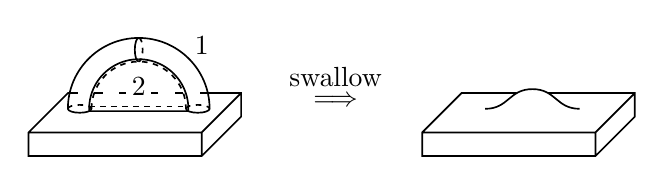
\begin{tikzpicture}[line width=.6]
    \tikzstyle{dp}=[dash pattern=on 2pt off 2pt]
    
    \draw (-.88,.2) -- (-.9,.2) -- (-1.4,-.3) -- (-1.4,-.6) -- (.8,-.6) -- (1.3,-.1) -- (1.3,.2) -- (.88,.2)
          (-1.4,-.3) -- (.8,-.3) -- (1.3,.2)
          (.8,-.3) -- (.8,-.6)
          (-.63,-.03) -- (.63,-.03);
    \draw[loosely dashed] (.88,.2) -- (0,.2) (-.88,.2) -- (0,.2);
    \draw[dp] (-.63,.03) -- (.63,.03);

    \draw[dp] (-.9,0) arc (180 : 0 : .15 and .05);
    \draw (-.9,0) arc (180 : 360 : .15 and .05);
    \draw[dp] (.6,0) arc (180 : 0 : .15 and .05);
    \draw (.6,0) arc (180 : 360 : .15 and .05);
    \draw[dp] (0,.9) arc (90 : -90 : .05 and .15);
    \draw (0,.9) arc (90 : 270 : .05 and .15);
    \draw (-.9,0) arc (180 : 0 : .9);
    \draw[dp] (-.6,0) arc (180 : 0 : .6);
    \draw (0,.63) arc (90 : -2 : .63);
    \draw (0,.63) arc (90 : 182 : .63);

    \node at (.8,.8) {1};
    \node[fill=white, inner xsep=2pt] at (0,.28) {2};

    \node at (2.5,.1) {\text{$\Longrightarrow$}};
    \node at (2.5,.4) {\text{swallow}};
    
    \draw (4.8,.2) -- (4.1,.2) -- (3.6,-.3) -- (3.6,-.6) -- (5.8,-.6) -- (6.3,-.1) -- (6.3,.2) -- (5.2,.2)
          (3.6,-.3) -- (5.8,-.3) -- (6.3,.2)
          (5.8,-.3) -- (5.8,-.6);
    \draw (4.4,0) .. controls (4.7,0) and (4.7,.25) .. (5,.25)
                  .. controls (5.3,.25) and (5.3,0) .. (5.6,0);
\end{tikzpicture} \]

For the proofs of these theorems,
see \cite{matsu} or \cite{milnor2}.
\medskip

Handlebodies are ubiquitous in the following sense.

\begin{theorem}\label{cor:handle-decomp}
    Every manifold is diffeomorphic to a good handlebody.
\end{theorem}

\begin{proof}
    \cite[Corollary~5.2.2]{wall}.
\end{proof}

However, some powerful tools, such as the rearrangement theorem,
fail for infinite handlebodies.
For example, consider the $2$-dimensional handlebody depicted below.
\[ 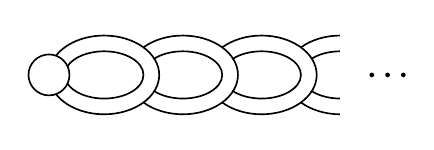
\begin{tikzpicture}[line width=.6]
    \draw (0,0) circle (.26);
    \draw (1.4,0) arc (0 : 151 : .7 and .5);
    \draw (1.4,0) arc (0 : -151 : .7 and .5);
    \draw (1.2,0) arc (0 : 159 : .5 and .3);
    \draw (1.2,0) arc (0 : -159 : .5 and .3);
    \draw (2.4,0) arc (0 : 136 : .7 and .5);
    \draw (2.4,0) arc (0 : -136 : .7 and .5);
    \draw (2.2,0) arc (0 : 138 : .5 and .3);
    \draw (2.2,0) arc (0 : -138 : .5 and .3);
    \draw (3.4,0) arc (0 : 136 : .7 and .5);
    \draw (3.4,0) arc (0 : -136 : .7 and .5);
    \draw (3.2,0) arc (0 : 138 : .5 and .3);
    \draw (3.2,0) arc (0 : -138 : .5 and .3);
    \draw (4.4,0) arc (0 : 136 : .7 and .5);
    \draw (4.4,0) arc (0 : -136 : .7 and .5);
    \draw (4.2,0) arc (0 : 138 : .5 and .3);
    \draw (4.2,0) arc (0 : -138 : .5 and .3);
    \fill[white] (3.7,.6) rectangle (4.5,-.6);
    \fill (4.1,0) circle (.03);
    \fill (4.3,0) circle (.03);
    \fill (4.5,0) circle (.03);
\end{tikzpicture} \]
If this handlebody were similar to a good handlebody,
then infinitely many $1$-handles would be attached
on the $0$-handle simultaneously,
so that the local finiteness criterion would fail.
In other words, if we attach handles in that way (pictured below),
we would get a topological space that is not a manifold.
\[ 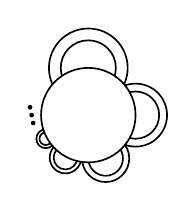
\begin{tikzpicture}[line width=.6]
    \draw[fill=white] (0,.6) circle (.5);
    \draw[fill=white] (0,.6) circle (.35);
    \draw[fill=white] (.6,0) circle (.4);
    \draw[fill=white] (.6,0) circle (.3);
    \draw[fill=white] (.22,-.55) circle (.3);
    \draw[fill=white] (.22,-.55) circle (.22);
    \draw[fill=white] (-.29,-.54) circle (.2);
    \draw[fill=white] (-.29,-.54) circle (.15);
    \draw[fill=white] (-.54,-.3) circle (.12);
    \draw[fill=white] (-.54,-.3) circle (.08);
    \draw[fill=white] (0,0) circle (.6);
    \fill (-.7, -.1) circle (.03);
    \fill (-.72, 0) circle (.03);
    \fill (-.74, .1) circle (.03);
\end{tikzpicture} \]

The purpose of this paper
is to introduce a variant of the notion of handlebodies,
which accepts this kind of spaces as handlebodies.
We will prove the rearrangement and cancellation theorems 
for this kind of handlebodies.
These results will make handle theory 
more available to non-compact manifolds.
